\usepackage{amsmath}
\usepackage{listings}
\usepackage{hyperref}
\usepackage{multicol}
\usepackage{graphicx}

\lstset{
  basicstyle=\footnotesize\ttfamily
}

% Version Info
% ------------
%
% * MAJOR.txt - Contains the major release version number.
% This will be updated to 2 when Embroidermodder 2 is final.
% Until then, it is set to 1 while Embroidermodder 2 is in development.
%
% * MINOR.txt - Contains the minor release version number.
% This file will be updated frequently when minor releases happen.
% It will be set to zero when Embroidermodder 2 is final.
% Until then, it is set to 90+ while Embroidermodder 2 is in development.
% The number shall be 2 digits, padded with a zero for single digit numbers.
%
% * PATCH.txt - Contains the patch release version number.
% This file will always be zero. Nightly builds will not use this file and
% will use the build unix date as such: ```date +%Y%m%d%H%M%S```
% This ensures that the latest build is always the highest number.

\newcommand{\emversion}{1.90.0}
\newcommand{\libembversion}{1.0.0}

\title{Embroidermodder User Manual}
\author{The Embroidermodder Team}

\begin{document}
\maketitle

\tableofcontents

\section{The Embroidermodder Project and Team}

The \emph{Embroidermodder 2} project is a collection of small software utilities for
manipulating, converting and creating embroidery files in all major embroidery
machine formats. The program \emph{Embroidermodder 2} itself is a larger graphical
user interface (GUI) which is at the heart of the project.

The tools and associated documents are:

\begin{itemize}
\item The website (www.libembroidery.org), which is maintained [docs-repo]_.
\item The manual [manual-link]_ covering all these projects which is maintained seperately as LaTeX [manual-src]_.
\item The GUI (embroidermodder), maintained \texttt{Embroidermodder 2}.
\item The core library of low-level functions: \texttt{libembroidery}.
\item The CLI `embroider` which is part of [libembroidery-src]_.
\item Mobile embroidery format viewers and tools [EmbroideryMobile-src]_.
\item Specs for an open hardware embroidery machine called Embroiderbot (not started yet) which is also part of [libembroidery-src]_.
\end{itemize}

.. [docs-repo] https://github.com/Embroidermodder/docs
.. [manual-link] https://www.libembroidery.org/embroidermodder_2.0_manual.pdf
.. [manual-src] https://github.com/Embroidermodder/emrm
.. [gui] https://github.com/Embroidermodder/embroidermodder
.. [libembroidery-src] https://github.com/Embroidermodder/libembroidery
.. [EmbroideryMobile-src] https://github.com/Embroidermodder/embroiderymobile

They are all tools to make the standard user experience of working with an
embroidery machine better without expensive software which is locked to specific
manufacturers and formats. But ultimately we hope that the core *Embroidermodder 2*
is a practical, ever-present tool in larger workshops, small cottage industry workshops
and personal hobbyist's bedrooms.

Embroidermodder 2 is licensed under the zlib license and we aim to keep all of
our tools open source and free of charge. If you would like to support the
project check out our `Open Collective <https://opencollective.com/embroidermodder>`_
group. If you would like to help, please
join us on GitHub. This document is written as developer training as well
helping new users (see the last sections) so this is the place to learn how
to start changing the code.

The Embroidermodder Team is the collection of people who've submitted
patches, artwork and documentation to our three projects.
The team was established by Jonathan Greig and Josh Varga.
The full list of contributors who wish to be credited is
here: https://www.libembroidery.org/docs/credits/

\subsection{Core Development Team}

Embroidermodder 2:

\begin{itemize}
\item Jonathan Greig \url{https://github.com/redteam316}
\item Josh Varga \url{https://github.com/JoshVarga}
\item Robin Swift [https://github.com/robin-swift](https://github.com/robin-swift)
\end{itemize}

Embroidermodder 1:

  * Josh Varga [https://github.com/JoshVarga](https://github.com/JoshVarga)
  * Mark Pontius [http://sourceforge.net/u/mpontius/profile](http://sourceforge.net/u/mpontius/profile)

## History

Embroidermodder 1 was started by Mark Pontius in 2004 while staying up all night
with his son in his first couple months. When Mark returned to his day job,
he lacked the time to continue the project. Mark made the decision to focus on his
family and work, and in 2005, Mark gave full control of the project to Josh Varga
so that Embroidermodder could continue its growth.

Embroidermodder 2 was conceived in mid 2011 when Jonathan Greig and Josh Varga
discussed the possibility of making a cross-platform version. It is currently in
active development and will run on GNU/Linux, Mac OS X, Microsoft Windows and Raspberry Pi.

The source code and binaries for Embroidermodder 1 were hosted on Sourceforge, but
due to link rot we've lost them.

!!! todo
    upload a backup here.

The source code for Embroidermodder
2 was moved to GitHub (\url{https://github.com/Embroidermodder/Embroidermodder})
on July 18, 2013.

This website was moved to
GitHub (\url{https://github.com/Embroidermodder/website}) on September 9, 2013. Due to us losing the domain name it was renamed to
\texttt{website} from \texttt{www.embroidermodder.org} and the new url \url{https://www.libembroidery.org}.

The libembroidery library (https://github.com/Embroidermodder/libembroidery)
became a seperate project in 2018 as a way of supporting other frontends with the
same file parsing and geometry routines.

\subsection{History}

Embroidermodder 1 was started by Mark Pontius in 2004 while staying up all night
with his son in his first couple months. When Mark returned to his day job, he
lacked the time to continue the project. Mark made the decision to focus on his
family and work, and in 2005, Mark gave full control of the project to Josh Varga
so that Embroidermodder could continue its growth.

Embroidermodder 2 was conceived in mid 2011 when Jonathan Greig and Josh Varga
discussed the possibility of making a cross-platform version. It is currently in
active development and will run on GNU/Linux, Mac OS X, Microsoft Windows and
Raspberry Pi.

The source code and binaries for Embroidermodder 1 were hosted on Sourceforge, but
due to link rot we've lost them.

!!! warning

    TODO: upload a backup here.

The `source code for Embroidermodder 2 <https://github.com/Embroidermodder/Embroidermodder>`_
was moved to GitHub on July 18, 2013.

`This website <https://github.com/Embroidermodder/docs>`_ was moved
to GitHub on September 9, 2013. Due to us losing the domain name it was renamed
to ``www.libembroidery.org`` from ``www.embroidermodder.org``.

The `libembroidery library <https://github.com/Embroidermodder/libembroidery>`_
became a seperate project in 2018 as a way of supporting other frontends with
the same file parsing and geometry routines.

\section{Batch Conversion}

\texttt{WARNING: THIS FEATURE IS NOT FUNCTIONAL, THIS SECTION IS PLANNING.}

Many users of \texttt{embroider} will only want our batch conversion feature.

\section{Changelog}

\subsection{From early alpha to beta}

\begin{itemize}
\item Up and Down keys cycle thru commands in the command prompt.
\end{itemize}

\section{Contributing}

\subsection{To Do}

\begin{itemize}
\item Copy of license in appendix.
\item Copy of manpage in appendix.
\end{itemize}

\begin{verbatim}
```
EMBROIDER(1)                 General Commands Manual                EMBROIDER(1)

NAME
       embroider - a command line program for machine embroidery

SYNOPSIS
       Copyright 2013-2023 The Embroidermodder Team Licensed under the terms of
       the zlib license.

       https://github.com/Embroidermodder/libembroidery
       https://www.libembroidery.org

       Usage: embroider [OPTIONS] fileToRead...

       Conversion:
           -t, --to        Convert all files given to the format specified
                           by the arguments to the flag, for example:
                               $ embroider -t dst input.pes
                           would convert
                           in the same directory the program runs in.

                           The accepted input formats are (TO BE DETERMINED).
                           The accepted output formats are (TO BE DETERMINED).

       Output:
           -h, --help       Print this message.
           -F, --formats     Print help on the formats that embroider can deal
       with.
           -q, --quiet      Only print fatal errors.
           -V, --verbose    Print everything that has reporting.
           -v, --version    Print the version.

       Modify patterns:
           --combine        takes 3 arguments and combines the first
                            two by placing them atop each other and
                            outputs to the third
                               $ embroider --combine a.dst b.dst output.dst

       Graphics:
           -c, --circle     Add a circle defined by the arguments given to the
       current pattern.
           -e, --ellipse    Add a circle defined by the arguments given to the
       current pattern.
           -l, --line       Add a line defined by the arguments given to the
       current pattern.
           -P, --polyline   Add a polyline.
           -p, --polygon    Add a polygon.
           -r, --render     Create an image in PNG format of what the embroidery
       should look like.
           -s, --satin      Fill the current geometry with satin stitches
       according
                            to the defined algorithm.
           -S, --stitch     Add a stitch defined by the arguments given to the
       current pattern.

       Quality Assurance:
               --test       Run the basic test suite.
               --full-test-suite  Run all tests, even those we expect to fail.

                                                                    EMBROIDER(1)
\end{verbatim}


\begin{verbatim}
EMBROIDER
    A command line program for machine embroidery.
    Copyright 2013-2021 The Embroidermodder Team
    Licensed under the terms of the zlib license.

    https://github.com/Embroidermodder/libembroidery
    https://embroidermodder.org

Usage: embroider [OPTIONS] fileToRead...

Conversion:
-t, -to         Convert all files given to the format specified
                by the arguments to the flag, for example:
                    $ embroider -t dst input.pes
                would convert \``input.pes\`` to \``input.dst\``
                in the same directory the program runs in.

                The accepted input formats are (TO BE DETERMINED).
                The accepted output formats are (TO BE DETERMINED).

Output:
-h, -help       Print this message.
-f, -format     Print help on the formats that
                embroider can deal with.
-q, -quiet      Only print fatal errors.
-V, -verbose    Print everything that has reporting.
-v, -version    Print the version.

Graphics:
-c, -circle     Add a circle defined by the arguments
                given to the current pattern.
-e, -ellipse    Add a circle defined by the arguments
                given to the current pattern.
-l, -line       Add a line defined by the arguments
                given to the current pattern.
-P, -polyline   Add a polyline.
-p, -polygon    Add a polygon.
-s, -satin      Fill the current geometry with satin
                stitches according
                to the defined algorithm.
-S, -stitch     Add a stitch defined by the arguments
                given to the current pattern.

Quality Assurance:
    -test       Run the test suite.# Full Colour Photograph, Vector and Black and White Designs

\end{verbatim}

WARNING: THIS FEATURE IS NOT AT ALL PRESENT, THIS SECTION IS PLANNING.

If you are starting an embroidery from an image, it's important to note that \embname uses very different
approaches based on what kind of image is fed into it. A photograph is the most difficult starting point
for an automated system since there are many artistic decisions which are mutually exclusive and
no software should make those decisions for you. At least, you should be aware that a decision is being made.
On the other hand, a vector based design gives the program the best starting point while still not being
a machine embroidery file. Finally a scan of a vector image or hand-drawn inkwork is somewhere in-between
these options and is the recommended option for people who work best on paper.

The following subsections are in order of how good the final results should be.

## Vector Designs
\index{vector}


## Scans of Hand-drawn Designs in a Limited Palette
\index{scans}


## Scans of Hand-drawn Designs in Block Colours
\index{scans}


## Full Colour Photographs
\index{photo}



\subsection{Command Line Generation}


\section{Embroidermodder on Mobile}

\section{Portable Embroidery Tool}

\section{Online Viewer and Converter}

!!! warning
    EXPERIMENTAL

\begin{verbatim}
<script>
  /* Call clang generated WASM here. */
  
</script>

If you only need to convert and view machine embroidery files (like our old Android application) then this page
does just that. To access other features of the Embroidermodder Project please see the [downloads.html](Downloads page).

<!-- Uses the native file dialog to get the string as a file object that is passed to a function from script above.
     If this is not called first, produce an error message. -->
<button onclick="upload();">Upload File</button>

<!-- Displays the SVG file output as a widget below. This could be by default. -->
<button onclick="show_svg();">Show</button>

<!-- Brings up the native file dialog, call "convert" with the arguments. -->
<button onclick="export_to();">Export...</button>

<svg class="viewer"></svg>
\end{verbatim}

This viewer uses no cookies and no external tools, so if you save this webpage to use offline it will still function.
Eventually, this webpage can be embedded in both an Android and an iOS app so we have, in total, 3 front-ends: embroider,
embroidermodder and the viewer/converter.

\section{Creating a Design}

WARNING: THIS FEATURE IS NOT FUNCTIONAL, THIS SECTION IS PLANNING.
# Credits for Embroidermodder 2, libembroidery and all other related code

Please note that this file in not in alphabetical order. If you have
contributed and wish to be added to this list, create a new credit
bullet. Fill it in with your information and submit it to us. Supply
your: your full name or pseudonym and GitHub handle, if available.

Kinds of contribution:

\begin{itemize}
\item Documentation - for changes to README files, manuals or help files.
\item Artwork - for artwork other than designs.
\item Bug Fixes - for small patches of a few lines.
\item Translation - for large patches to the translation files.
\item Designs - for an embroidery design sample or parametrized design as a toml file.
\item Bindings - for programming language bindings for libembroidery.
\item Commands - for Embroidermodder 2's in-built terminal.
\end{itemize}

finally there's \textbf{Core Developer} which is reserved for long term
contributors.

\subsection{Contributors}

!!! warning
    Need to fix script to generate from ``data``.

\section{Editing Designs}

WARNING: THIS FEATURE IS NOT FUNCTIONAL, THIS SECTION IS PLANNING.

\subsection{Command Line Editing}

\section{Introduction}

title: The Embroidermodder Project
description: Free and Open Source Software for Machine Embroidery.
keywords: machine embroidery, embroidery, dst, pes, jef

WARNING  ( IN ALPHA DEVELOPMENT: NOT YET READY FOR SERIOUS USE. )

Embroidermodder is a free machine embroidery software program.
The newest version, Embroidermodder 2 can:

- edit and create embroidery designs
- estimate the amount of thread and machine time needed to stitch a design
- convert embroidery files to a variety of formats
- upscale or downscale designs
- run on Windows, Mac and Linux

For more in-depth information, see [our website](http://www.libembroidery.org)
and get the manuals [here](http://www.libembroidery.org/documentation).

To try out the software in alpha see our current
[alpha pre-release](https://github.com/Embroidermodder/Embroidermodder/releases).

Various sample embroidery design files can be found in
the src/samples folder.

Embroidermodder is developed by The Embroidermodder Team which is maintained as a
list on the website under ["Credits"](http://www.libembroidery.org/credits).

## Screenshots

If you use multiple operating systems, it's important to choose software that works on all of them.

Embroidermodder 2 runs on Windows, Linux and Mac OS X. Let's not forget the [Raspberry
Pi](http://www.raspberrypi.org).

![features: platforms 1](images/features-platforms-1.png)

### Realistic Rendering

(This feature is currently broken.)

It is important to be able to visualize what a design will look like when stitched and our
pseudo ``3D'' realistic rendering helps achieve this.

Realistic rendering sample \#1:

![features real render 1](images/features-realrender-1.png)

Realistic rendering sample \#2:

![features real render 2](images/features-realrender-2.png)

Realistic rendering sample \#3:

![features real render 3](images/features-realrender-3.png)

Various grid types and auto-adjusting rulers

Making use of the automatically adjusting ruler in conjunction with the grid will ensure your
design is properly sized and fits within your embroidery hoop area.

Use rectangular, circular or isometric grids to construct your masterpiece!

Multiple grids and rulers in action:

![features grid ruler](images/features-grid-ruler-1.png)

### Many measurement tools

Taking measurements is a critical part of creating great designs. Whether you are designing
mission critical embroidered space suits for NASA or some other far out design for your next
meet-up, you will have precise measurement tools at your command to make it happen. You can
locate individual points or find distances between any 2 points anywhere in the design!

Take quick and accurate measurements:

![features measure 1](images/features-measure-1.png)

### Add text to any design

Need to make company apparel for all of your employees with individual names on them? No sweat.
Just simply add text to your existing design or create one from scratch, quickly and easily.
Didn't get it the right size or made a typo? No problem. Just select the text and update it
with the property editor.

Add text and adjust its properties quickly:

![features text 1](images/features-text-1.png)

### Supports many formats

Embroidery machines all accept different formats. There are so many formats available that it
can sometimes be confusing whether a design will work with your machine.

Embroidermodder 2 supports a wide variety of embroidery formats as well as several vector
formats, such as SVG and DXF. This allows you to worry less about which designs you can use.

\subsubsection{Batch Conversion}

(Currently this being ported to the \texttt{embroider} command line program.)

Need to send a client several different formats? Just use libembroidery-convert, our command
line utility which supports batch file conversion.

There are a multitude of formats to choose from:

\begin{figure}[H]
\centering}
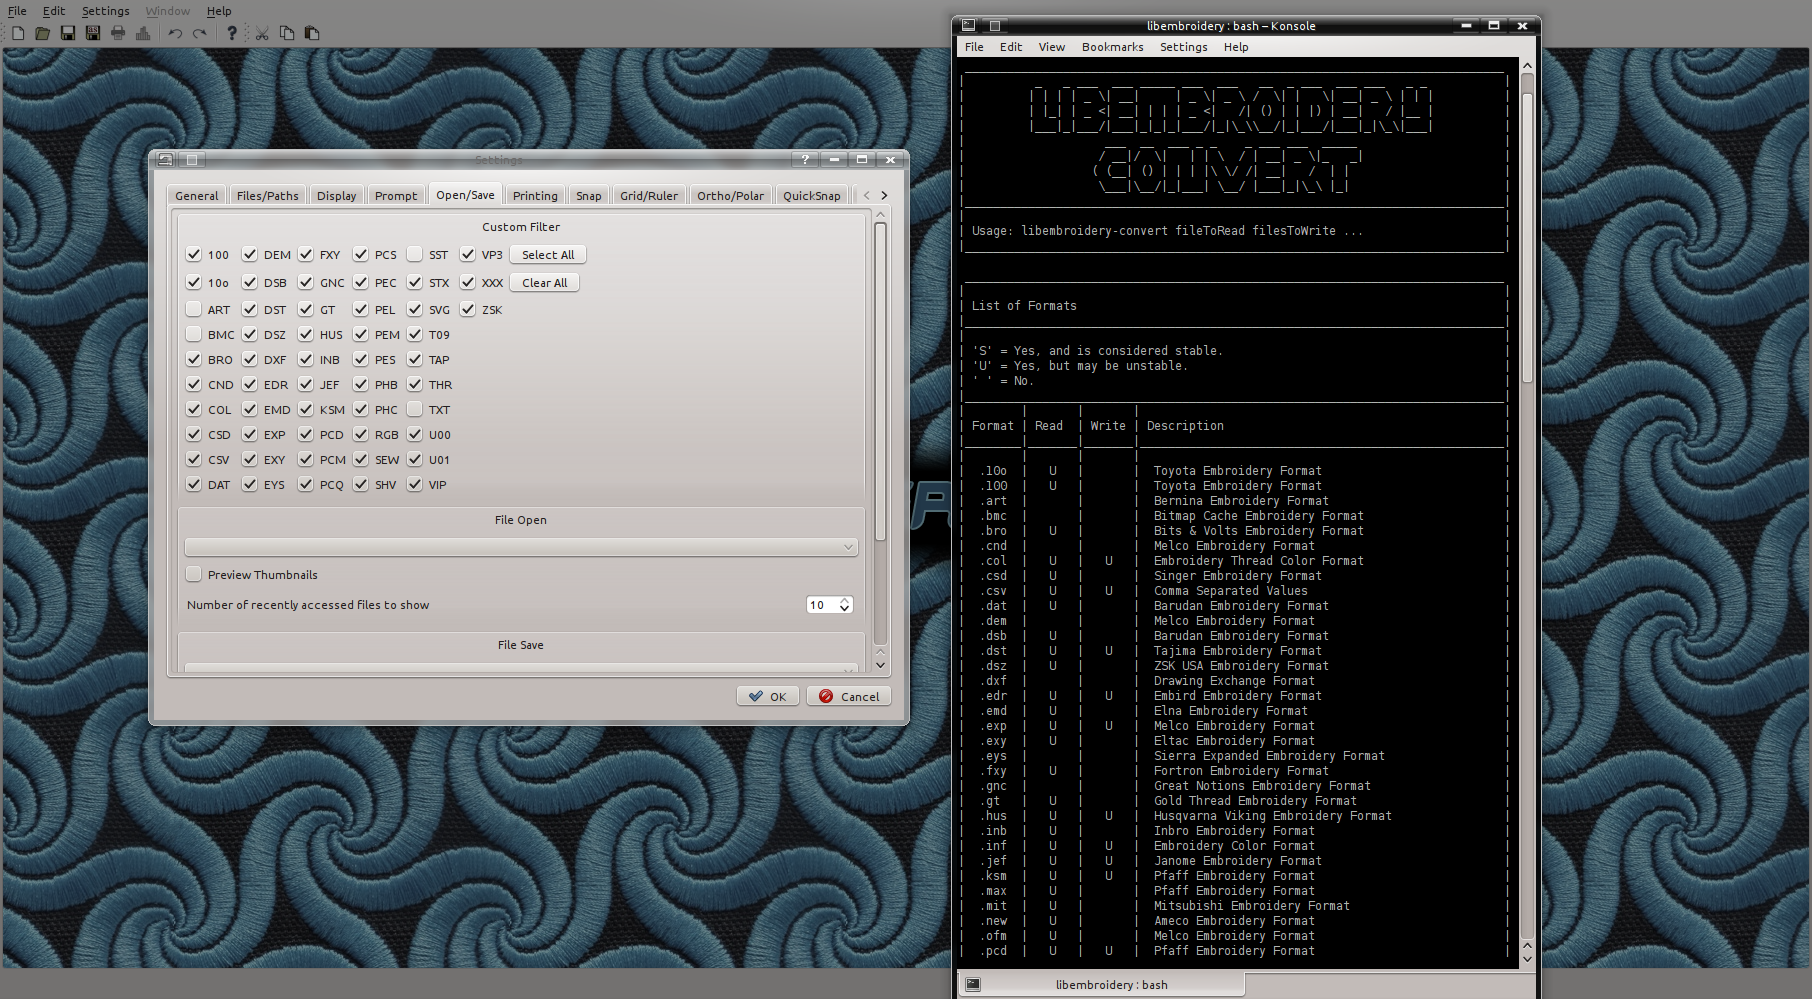
\includegraphics[width=0.8\textwidth]{images/features-formats-1.png}
\caption{features formats}
\end{figure}

\subsubsection{Scripting API}

The GUI works by emitting internal text commands, so if you want to alter
or add features to the program that aren't as low level as these commands then you
can chain them together in simple scripts. This allows more control over the program than
the GUI can offer.

A (no longer current) Embroidermodder 2 command excerpt:

\begin{figure}[H]
\centering
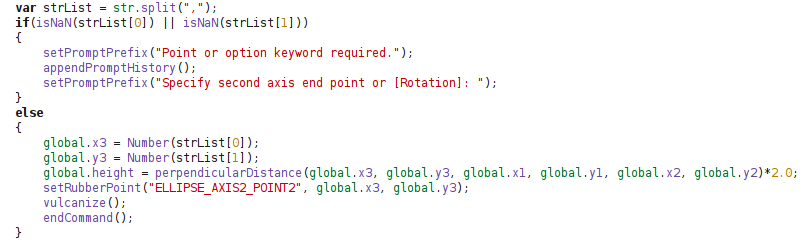
\includegraphics[width=0.8\textwidth]{images/features-scripting-1.png}
\caption{scripting screenshot}
\end{figure}

\subsection{Dependencies}

To build Embroidermodder 2 from source you will need at least
[the Embroidermodder 2 source code itself](https://github.com/Embroidermodder/Embroidermodder),
a build environment including [CMake](https://cmake.org) and [Qt](http://www.qt-project.org) (version >= 6.0). For advice on how to get these,
see the following subsections.

You will also need the git submodules, which can be collected by running these lines
from the embroidermodder source directory:

```
git submodule init
git submodule update
```

### Debian/Ubuntu repository packages

The Qt, KDE and Valgrind build dependencies can be installed easily by
opening a terminal and issuing these commands:

```
sudo apt-get update
sudo apt-get install cmake build-essential qt6-base-dev libqt6gui6 libqt6widgets6 libqt6printsupport6 libqt6core6 libgl-dev libglx-dev libopengl-dev
```

### Fedora repository packages

_TODO: This is outdated advice._

The Qt, KDE and Valgrind build dependencies can be installed easily
by opening a terminal and issuing this command:

```
sudo yum install git gdb gcc-c++ qt-devel kdelibs-devel valgrind
```

\subsubsection{Windows (MSYS2)}

After installing [MSYS2](https://www.msys2.org), run this command in a MINGW64 shell:

```sh
pacman -S mingw-w64-clang-x86_64-qt6 cmake gcc make git
```

At the time of writing, this will use around 2Gb of disk space. Then continue to [build](#build).

\subsubsection{Windows (Without MinGW or MSYS2)}

If you have a development environment and for some reason want to use that over MSYS2 then ensure you run the installers for:

1. CMake: https://cmake.org/download/#latest
2. Qt: http://www.qt-project.org
3. A Text Editor for Code like Visual Studio Code: https://code.visualstudio.com/
4. A C compiler, like `gcc`, `cl`, `clang` or `tcc`.
5. Git Bash: https://gitforwindows.org/
6. A backend for CMake like Ninja: https://ninja-build.org/

Remember to add these to your `PATH` for scripts to use them.

This would give a similar build experience to standard development on Windows, but we recommend you use MSYS2.

Note that our behind-the-scenes Windows build uses Python to get the Qt libraries
[like this](https://github.com/Embroidermodder/libembroidery/blob/main/bin/build.sh).

\subsection{Build}

Assuming you have the dependencies for your system, on all systems with Bash, the following should work:

\begin{lstlisting}
bash build.sh
\end{lstlisting}

If your system does not have bash, it may still run as sh.
Failing that, try typing each line in in turn like this:

\begin{lstlisting}
git submodule init
git submodule update

cmake -S . -B"build" -G"Unix Makefiles" -DCMAKE_BUILD_TYPE="Debug"
cd build
cp -r ../assets/* .
cmake --build .
cat build.log
cd ..
\end{lstlisting}

\subsubsection{Running the Development Version}

After building as above, run your own development copy with:

\begin{lstlisting}
cd build
./embroidermodder2
\end{lstlisting}

\subsubsection{Troubleshooting}

If you have no luck with the above advice and still want to
run the development alpha, try reading the `build.log` in your
`build/` folder like this:

```sh
cat build/build.log
```

If, after googling keywords from the errors you're still stuck
post and issue on GitHub here: https://github.com/Embroidermodder/Embroidermodder/issues and supply the `build.log` file. If something
comes up a lot then we can add advice here.

## Development

During the alpha phase we mainly need to focus on getting the C bedrock of this project stable before letting more people
put their creations into it. In Beta, non-programming related contributions will be wecomed to the website and reference manual
repositories.

### Getting Involved

Anyone interested in changing Embroidermodder or becoming a contributor should go read our
[manuals](https://libembroidery.org/documentation), [make issues and submit patches](https://github.com/embroidermodder/refman)
as you find them because the project is very weak here. It will also serve as training for submitting patches to the actual
source code where changes are harder to critique and revise.

As for helping with specific bugs submitting an issue on GitHub along with the `debug-####.txt` file generated during
your test run would be the best approach. For longer term techniques see the next section.

### Bug Hunting

The Embroidermodder Project
===========================

.. toctree::
   :maxdepth: 2
   :caption: Contents
   :name: maintoc

   em_user
   mobile_user
   pet_user
   emrm
   credits

.. warning::

   IN ALPHA DEVELOPMENT: NOT READY FOR SERIOUS USE.

Embroidermodder is a free and open source machine embroidery application.
If our project is successful, it will:

\begin{itemize}
\item edit and create embroidery designs
\item estimate the amount of thread and machine time needed to stitch a design
\item convert embroidery files to a variety of formats
\item upscale or downscale designs
\item run on Windows, Mac and Linux
\end{itemize}

To try out the software in alpha see our `downloads page <https://libembroidery.org/downloads>`_.

Various sample embroidery design files can be found in
the github samples folder.

Screenshots
-----------

If you use multiple operating systems, it's important to choose
software that works on all of them. Embroidermodder 2 runs on Windows,
Linux and Mac OS X. Let's not forget the `Raspberry Pi <https://www.raspberrypi.org>`_.

\section{Documentation}

For all of these manuals (except the `embroider` manpage),
the source code is maintained as part
of the website [here](https://github.com/Embroidermodder/docs).

\subsection{The User Manuals}

Note that these URLs are maintained as the permalinks.

For all of these user manuals including the ``embroider`` manpage,
the source code is maintained as part
of the libembroidery project ([https://github.com/Embroidermodder/libembroidery](https://github.com/Embroidermodder/libembroidery)).
The documentation, like the code, is mostly common to all subprojects.

\begin{itemize}
\item Embroidermodder, EmbroideryMobile, PET: [https://www.libembroidery.org/user-manual](https://www.libembroidery.org/user-manual) ([PDF](https://www.libembroidery.org/em2_user_manual.pdf))
\item embroider: [https://www.libembroidery.org/embroider.txt](https://www.libembroidery.org/embroider.txt)
\end{itemize}

\subsection{The Developer Manual}

The Embroidermodder Reference Manual (EMRM) is the main developer 
resource found here: [https://www.libembroidery.org/refman](https://www.libembroidery.org/refman) with the printer friendly version here: [https://www.libembroidery.org/downloads/emrm.pdf](https://www.libembroidery.org/downloads/emrm.pdf).

\section{The Embroidermodder Project Website}

This directory contains most of the broader documentation and automation to
stop minor changes flooding each of Embroidermodder's sub-projects. Including
the documentation as webpages for the
[site itself](https://www.libembroidery.org), each subproject's user manual but
not the reference manual.

This frees the other repositories of the minor-commit heavy mundane tasks of
bundling software and separating a "user" build from a "production" build. It
also means that those projects aren't tasked with keeping production history.

For in-depth information about the software please read some of the PDF manual
included in the top level of the repository. Finishing the manual is the current
top priority in order to fascilitate new developers joining the project.

\subsection{Ideas}

A testing site that is maintained under testing.libembroidery.org so builds
don't go straight to the main landing page.

If this reaches the cap of storage offered by a github repository then we'll
have to think of something else since the version history of the binaries could
quickly become important if we have any regressions.

\section{Embroidermodder 2.0.0-alpha4  User Manual}

\subsection{Introduction}

!!! warning
    THIS MANUAL IS IN PROGRESS: PLEASE WAIT FOR THE BETA RELEASE.

This manual is for the various ways of using the \embname tools for designing,
editing and converting machine embroidery files. Most users should try loading and altering a design
in \embname itself before trying any of our conversion tools, our embedded system
or the command line interface. Advice on this is in the next section.

If you wish to write your own
software that uses these tools you will need the \embname Reference Manual (this
includes the API documentation). This is maintained at the permalink
\url{https://www.libembroidery.org/downloads/emrm.pdf}.

\begin{multicols}{2}
\footnotesize
\section{License}

\hfuzz = .6pt % avoid black boxes

%---------------------------------------------------------------------
\chapter*{\rlap{GNU Free Documentation License}}
\phantomsection  % so hyperref creates bookmarks
\addcontentsline{toc}{chapter}{GNU Free Documentation License}
%\label{label_fdl}

 \begin{center}

       Version 1.3, 3 November 2008


 Copyright \copyright{} 2000, 2001, 2002, 2007, 2008  Free Software Foundation, Inc.
 
 \bigskip
 
     \texttt{<https://fsf.org/>}
  
 \bigskip
 
 Everyone is permitted to copy and distribute verbatim copies
 of this license document, but changing it is not allowed.
\end{center}


\begin{center}
{\bf\large Preamble}
\end{center}

The purpose of this License is to make a manual, textbook, or other
functional and useful document ``free'' in the sense of freedom: to
assure everyone the effective freedom to copy and redistribute it,
with or without modifying it, either commercially or noncommercially.
Secondarily, this License preserves for the author and publisher a way
to get credit for their work, while not being considered responsible
for modifications made by others.

This License is a kind of ``copyleft'', which means that derivative
works of the document must themselves be free in the same sense.  It
complements the GNU General Public License, which is a copyleft
license designed for free software.

We have designed this License in order to use it for manuals for free
software, because free software needs free documentation: a free
program should come with manuals providing the same freedoms that the
software does.  But this License is not limited to software manuals;
it can be used for any textual work, regardless of subject matter or
whether it is published as a printed book.  We recommend this License
principally for works whose purpose is instruction or reference.


\begin{center}
{\Large\bf 1. APPLICABILITY AND DEFINITIONS\par}
\phantomsection
\addcontentsline{toc}{section}{1. APPLICABILITY AND DEFINITIONS}
\end{center}

This License applies to any manual or other work, in any medium, that
contains a notice placed by the copyright holder saying it can be
distributed under the terms of this License.  Such a notice grants a
world-wide, royalty-free license, unlimited in duration, to use that
work under the conditions stated herein.  The ``\textbf{Document}'', below,
refers to any such manual or work.  Any member of the public is a
licensee, and is addressed as ``\textbf{you}''.  You accept the license if you
copy, modify or distribute the work in a way requiring permission
under copyright law.

A ``\textbf{Modified Version}'' of the Document means any work containing the
Document or a portion of it, either copied verbatim, or with
modifications and/or translated into another language.

A ``\textbf{Secondary Section}'' is a named appendix or a front-matter section of
the Document that deals exclusively with the relationship of the
publishers or authors of the Document to the Document's overall subject
(or to related matters) and contains nothing that could fall directly
within that overall subject.  (Thus, if the Document is in part a
textbook of mathematics, a Secondary Section may not explain any
mathematics.)  The relationship could be a matter of historical
connection with the subject or with related matters, or of legal,
commercial, philosophical, ethical or political position regarding
them.

The ``\textbf{Invariant Sections}'' are certain Secondary Sections whose titles
are designated, as being those of Invariant Sections, in the notice
that says that the Document is released under this License.  If a
section does not fit the above definition of Secondary then it is not
allowed to be designated as Invariant.  The Document may contain zero
Invariant Sections.  If the Document does not identify any Invariant
Sections then there are none.

The ``\textbf{Cover Texts}'' are certain short passages of text that are listed,
as Front-Cover Texts or Back-Cover Texts, in the notice that says that
the Document is released under this License.  A Front-Cover Text may
be at most 5 words, and a Back-Cover Text may be at most 25 words.

A ``\textbf{Transparent}'' copy of the Document means a machine-readable copy,
represented in a format whose specification is available to the
general public, that is suitable for revising the document
straightforwardly with generic text editors or (for images composed of
pixels) generic paint programs or (for drawings) some widely available
drawing editor, and that is suitable for input to text formatters or
for automatic translation to a variety of formats suitable for input
to text formatters.  A copy made in an otherwise Transparent file
format whose markup, or absence of markup, has been arranged to thwart
or discourage subsequent modification by readers is not Transparent.
An image format is not Transparent if used for any substantial amount
of text.  A copy that is not ``Transparent'' is called ``\textbf{Opaque}''.

Examples of suitable formats for Transparent copies include plain
ASCII without markup, Texinfo input format, LaTeX input format, SGML
or XML using a publicly available DTD, and standard-conforming simple
HTML, PostScript or PDF designed for human modification.  Examples of
transparent image formats include PNG, XCF and JPG.  Opaque formats
include proprietary formats that can be read and edited only by
proprietary word processors, SGML or XML for which the DTD and/or
processing tools are not generally available, and the
machine-generated HTML, PostScript or PDF produced by some word
processors for output purposes only.

The ``\textbf{Title Page}'' means, for a printed book, the title page itself,
plus such following pages as are needed to hold, legibly, the material
this License requires to appear in the title page.  For works in
formats which do not have any title page as such, ``Title Page'' means
the text near the most prominent appearance of the work's title,
preceding the beginning of the body of the text.

The ``\textbf{publisher}'' means any person or entity that distributes
copies of the Document to the public.

A section ``\textbf{Entitled XYZ}'' means a named subunit of the Document whose
title either is precisely XYZ or contains XYZ in parentheses following
text that translates XYZ in another language.  (Here XYZ stands for a
specific section name mentioned below, such as ``\textbf{Acknowledgements}'',
``\textbf{Dedications}'', ``\textbf{Endorsements}'', or ``\textbf{History}''.)  
To ``\textbf{Preserve the Title}''
of such a section when you modify the Document means that it remains a
section ``Entitled XYZ'' according to this definition.

The Document may include Warranty Disclaimers next to the notice which
states that this License applies to the Document.  These Warranty
Disclaimers are considered to be included by reference in this
License, but only as regards disclaiming warranties: any other
implication that these Warranty Disclaimers may have is void and has
no effect on the meaning of this License.


\begin{center}
{\Large\bf 2. VERBATIM COPYING\par}
\phantomsection
\addcontentsline{toc}{section}{2. VERBATIM COPYING}
\end{center}

You may copy and distribute the Document in any medium, either
commercially or noncommercially, provided that this License, the
copyright notices, and the license notice saying this License applies
to the Document are reproduced in all copies, and that you add no other
conditions whatsoever to those of this License.  You may not use
technical measures to obstruct or control the reading or further
copying of the copies you make or distribute.  However, you may accept
compensation in exchange for copies.  If you distribute a large enough
number of copies you must also follow the conditions in section~3.

You may also lend copies, under the same conditions stated above, and
you may publicly display copies.


\begin{center}
{\Large\bf 3. COPYING IN QUANTITY\par}
\phantomsection
\addcontentsline{toc}{section}{3. COPYING IN QUANTITY}
\end{center}


If you publish printed copies (or copies in media that commonly have
printed covers) of the Document, numbering more than 100, and the
Document's license notice requires Cover Texts, you must enclose the
copies in covers that carry, clearly and legibly, all these Cover
Texts: Front-Cover Texts on the front cover, and Back-Cover Texts on
the back cover.  Both covers must also clearly and legibly identify
you as the publisher of these copies.  The front cover must present
the full title with all words of the title equally prominent and
visible.  You may add other material on the covers in addition.
Copying with changes limited to the covers, as long as they preserve
the title of the Document and satisfy these conditions, can be treated
as verbatim copying in other respects.

If the required texts for either cover are too voluminous to fit
legibly, you should put the first ones listed (as many as fit
reasonably) on the actual cover, and continue the rest onto adjacent
pages.

If you publish or distribute Opaque copies of the Document numbering
more than 100, you must either include a machine-readable Transparent
copy along with each Opaque copy, or state in or with each Opaque copy
a computer-network location from which the general network-using
public has access to download using public-standard network protocols
a complete Transparent copy of the Document, free of added material.
If you use the latter option, you must take reasonably prudent steps,
when you begin distribution of Opaque copies in quantity, to ensure
that this Transparent copy will remain thus accessible at the stated
location until at least one year after the last time you distribute an
Opaque copy (directly or through your agents or retailers) of that
edition to the public.

It is requested, but not required, that you contact the authors of the
Document well before redistributing any large number of copies, to give
them a chance to provide you with an updated version of the Document.


\begin{center}
{\Large\bf 4. MODIFICATIONS\par}
\phantomsection
\addcontentsline{toc}{section}{4. MODIFICATIONS}
\end{center}

You may copy and distribute a Modified Version of the Document under
the conditions of sections 2 and 3 above, provided that you release
the Modified Version under precisely this License, with the Modified
Version filling the role of the Document, thus licensing distribution
and modification of the Modified Version to whoever possesses a copy
of it.  In addition, you must do these things in the Modified Version:

\begin{itemize}
\item[A.] 
   Use in the Title Page (and on the covers, if any) a title distinct
   from that of the Document, and from those of previous versions
   (which should, if there were any, be listed in the History section
   of the Document).  You may use the same title as a previous version
   if the original publisher of that version gives permission.
   
\item[B.]
   List on the Title Page, as authors, one or more persons or entities
   responsible for authorship of the modifications in the Modified
   Version, together with at least five of the principal authors of the
   Document (all of its principal authors, if it has fewer than five),
   unless they release you from this requirement.
   
\item[C.]
   State on the Title page the name of the publisher of the
   Modified Version, as the publisher.
   
\item[D.]
   Preserve all the copyright notices of the Document.
   
\item[E.]
   Add an appropriate copyright notice for your modifications
   adjacent to the other copyright notices.
   
\item[F.]
   Include, immediately after the copyright notices, a license notice
   giving the public permission to use the Modified Version under the
   terms of this License, in the form shown in the Addendum below.
   
\item[G.]
   Preserve in that license notice the full lists of Invariant Sections
   and required Cover Texts given in the Document's license notice.
   
\item[H.]
   Include an unaltered copy of this License.
   
\item[I.]
   Preserve the section Entitled ``History'', Preserve its Title, and add
   to it an item stating at least the title, year, new authors, and
   publisher of the Modified Version as given on the Title Page.  If
   there is no section Entitled ``History'' in the Document, create one
   stating the title, year, authors, and publisher of the Document as
   given on its Title Page, then add an item describing the Modified
   Version as stated in the previous sentence.
   
\item[J.]
   Preserve the network location, if any, given in the Document for
   public access to a Transparent copy of the Document, and likewise
   the network locations given in the Document for previous versions
   it was based on.  These may be placed in the ``History'' section.
   You may omit a network location for a work that was published at
   least four years before the Document itself, or if the original
   publisher of the version it refers to gives permission.
   
\item[K.]
   For any section Entitled ``Acknowledgements'' or ``Dedications'',
   Preserve the Title of the section, and preserve in the section all
   the substance and tone of each of the contributor acknowledgements
   and/or dedications given therein.
   
\item[L.]
   Preserve all the Invariant Sections of the Document,
   unaltered in their text and in their titles.  Section numbers
   or the equivalent are not considered part of the section titles.
   
\item[M.]
   Delete any section Entitled ``Endorsements''.  Such a section
   may not be included in the Modified Version.
   
\item[N.]
   Do not retitle any existing section to be Entitled ``Endorsements''
   or to conflict in title with any Invariant Section.
   
\item[O.]
   Preserve any Warranty Disclaimers.
\end{itemize}

If the Modified Version includes new front-matter sections or
appendices that qualify as Secondary Sections and contain no material
copied from the Document, you may at your option designate some or all
of these sections as invariant.  To do this, add their titles to the
list of Invariant Sections in the Modified Version's license notice.
These titles must be distinct from any other section titles.

You may add a section Entitled ``Endorsements'', provided it contains
nothing but endorsements of your Modified Version by various
parties---for example, statements of peer review or that the text has
been approved by an organization as the authoritative definition of a
standard.

You may add a passage of up to five words as a Front-Cover Text, and a
passage of up to 25 words as a Back-Cover Text, to the end of the list
of Cover Texts in the Modified Version.  Only one passage of
Front-Cover Text and one of Back-Cover Text may be added by (or
through arrangements made by) any one entity.  If the Document already
includes a cover text for the same cover, previously added by you or
by arrangement made by the same entity you are acting on behalf of,
you may not add another; but you may replace the old one, on explicit
permission from the previous publisher that added the old one.

The author(s) and publisher(s) of the Document do not by this License
give permission to use their names for publicity for or to assert or
imply endorsement of any Modified Version.


\begin{center}
{\Large\bf 5. COMBINING DOCUMENTS\par}
\phantomsection
\addcontentsline{toc}{section}{5. COMBINING DOCUMENTS}
\end{center}


You may combine the Document with other documents released under this
License, under the terms defined in section~4 above for modified
versions, provided that you include in the combination all of the
Invariant Sections of all of the original documents, unmodified, and
list them all as Invariant Sections of your combined work in its
license notice, and that you preserve all their Warranty Disclaimers.

The combined work need only contain one copy of this License, and
multiple identical Invariant Sections may be replaced with a single
copy.  If there are multiple Invariant Sections with the same name but
different contents, make the title of each such section unique by
adding at the end of it, in parentheses, the name of the original
author or publisher of that section if known, or else a unique number.
Make the same adjustment to the section titles in the list of
Invariant Sections in the license notice of the combined work.

In the combination, you must combine any sections Entitled ``History''
in the various original documents, forming one section Entitled
``History''; likewise combine any sections Entitled ``Acknowledgements'',
and any sections Entitled ``Dedications''.  You must delete all sections
Entitled ``Endorsements''.

\begin{center}
{\Large\bf 6. COLLECTIONS OF DOCUMENTS\par}
\phantomsection
\addcontentsline{toc}{section}{6. COLLECTIONS OF DOCUMENTS}
\end{center}

You may make a collection consisting of the Document and other documents
released under this License, and replace the individual copies of this
License in the various documents with a single copy that is included in
the collection, provided that you follow the rules of this License for
verbatim copying of each of the documents in all other respects.

You may extract a single document from such a collection, and distribute
it individually under this License, provided you insert a copy of this
License into the extracted document, and follow this License in all
other respects regarding verbatim copying of that document.


\begin{center}
{\Large\bf 7. AGGREGATION WITH INDEPENDENT WORKS\par}
\phantomsection
\addcontentsline{toc}{section}{7. AGGREGATION WITH INDEPENDENT WORKS}
\end{center}


A compilation of the Document or its derivatives with other separate
and independent documents or works, in or on a volume of a storage or
distribution medium, is called an ``aggregate'' if the copyright
resulting from the compilation is not used to limit the legal rights
of the compilation's users beyond what the individual works permit.
When the Document is included in an aggregate, this License does not
apply to the other works in the aggregate which are not themselves
derivative works of the Document.

If the Cover Text requirement of section~3 is applicable to these
copies of the Document, then if the Document is less than one half of
the entire aggregate, the Document's Cover Texts may be placed on
covers that bracket the Document within the aggregate, or the
electronic equivalent of covers if the Document is in electronic form.
Otherwise they must appear on printed covers that bracket the whole
aggregate.


\begin{center}
{\Large\bf 8. TRANSLATION\par}
\phantomsection
\addcontentsline{toc}{section}{8. TRANSLATION}
\end{center}


Translation is considered a kind of modification, so you may
distribute translations of the Document under the terms of section~4.
Replacing Invariant Sections with translations requires special
permission from their copyright holders, but you may include
translations of some or all Invariant Sections in addition to the
original versions of these Invariant Sections.  You may include a
translation of this License, and all the license notices in the
Document, and any Warranty Disclaimers, provided that you also include
the original English version of this License and the original versions
of those notices and disclaimers.  In case of a disagreement between
the translation and the original version of this License or a notice
or disclaimer, the original version will prevail.

If a section in the Document is Entitled ``Acknowledgements'',
``Dedications'', or ``History'', the requirement (section~4) to Preserve
its Title (section~1) will typically require changing the actual
title.


\begin{center}
{\Large\bf 9. TERMINATION\par}
\phantomsection
\addcontentsline{toc}{section}{9. TERMINATION}
\end{center}


You may not copy, modify, sublicense, or distribute the Document
except as expressly provided under this License.  Any attempt
otherwise to copy, modify, sublicense, or distribute it is void, and
will automatically terminate your rights under this License.

However, if you cease all violation of this License, then your license
from a particular copyright holder is reinstated (a) provisionally,
unless and until the copyright holder explicitly and finally
terminates your license, and (b) permanently, if the copyright holder
fails to notify you of the violation by some reasonable means prior to
60 days after the cessation.

Moreover, your license from a particular copyright holder is
reinstated permanently if the copyright holder notifies you of the
violation by some reasonable means, this is the first time you have
received notice of violation of this License (for any work) from that
copyright holder, and you cure the violation prior to 30 days after
your receipt of the notice.

Termination of your rights under this section does not terminate the
licenses of parties who have received copies or rights from you under
this License.  If your rights have been terminated and not permanently
reinstated, receipt of a copy of some or all of the same material does
not give you any rights to use it.


\begin{center}
{\Large\bf 10. FUTURE REVISIONS OF THIS LICENSE\par}
\phantomsection
\addcontentsline{toc}{section}{10. FUTURE REVISIONS OF THIS LICENSE}
\end{center}


The Free Software Foundation may publish new, revised versions
of the GNU Free Documentation License from time to time.  Such new
versions will be similar in spirit to the present version, but may
differ in detail to address new problems or concerns.  See
\texttt{https://www.gnu.org/licenses/}.

Each version of the License is given a distinguishing version number.
If the Document specifies that a particular numbered version of this
License ``or any later version'' applies to it, you have the option of
following the terms and conditions either of that specified version or
of any later version that has been published (not as a draft) by the
Free Software Foundation.  If the Document does not specify a version
number of this License, you may choose any version ever published (not
as a draft) by the Free Software Foundation.  If the Document
specifies that a proxy can decide which future versions of this
License can be used, that proxy's public statement of acceptance of a
version permanently authorizes you to choose that version for the
Document.


\begin{center}
{\Large\bf 11. RELICENSING\par}
\phantomsection
\addcontentsline{toc}{section}{11. RELICENSING}
\end{center}


``Massive Multiauthor Collaboration Site'' (or ``MMC Site'') means any
World Wide Web server that publishes copyrightable works and also
provides prominent facilities for anybody to edit those works.  A
public wiki that anybody can edit is an example of such a server.  A
``Massive Multiauthor Collaboration'' (or ``MMC'') contained in the
site means any set of copyrightable works thus published on the MMC
site.

``CC-BY-SA'' means the Creative Commons Attribution-Share Alike 3.0
license published by Creative Commons Corporation, a not-for-profit
corporation with a principal place of business in San Francisco,
California, as well as future copyleft versions of that license
published by that same organization.

``Incorporate'' means to publish or republish a Document, in whole or
in part, as part of another Document.

An MMC is ``eligible for relicensing'' if it is licensed under this
License, and if all works that were first published under this License
somewhere other than this MMC, and subsequently incorporated in whole
or in part into the MMC, (1) had no cover texts or invariant sections,
and (2) were thus incorporated prior to November 1, 2008.

The operator of an MMC Site may republish an MMC contained in the site
under CC-BY-SA on the same site at any time before August 1, 2009,
provided the MMC is eligible for relicensing.


\begin{center}
{\Large\bf ADDENDUM: How to use this License for your documents\par}
\phantomsection
\addcontentsline{toc}{section}{ADDENDUM: How to use this License for your documents}
\end{center}

To use this License in a document you have written, include a copy of
the License in the document and put the following copyright and
license notices just after the title page:

\bigskip
\begin{quote}
    Copyright \copyright{}  YEAR  YOUR NAME.
    Permission is granted to copy, distribute and/or modify this document
    under the terms of the GNU Free Documentation License, Version 1.3
    or any later version published by the Free Software Foundation;
    with no Invariant Sections, no Front-Cover Texts, and no Back-Cover Texts.
    A copy of the license is included in the section entitled ``GNU
    Free Documentation License''.
\end{quote}
\bigskip
    
If you have Invariant Sections, Front-Cover Texts and Back-Cover Texts,
replace the ``with \dots\ Texts.''\ line with this:

\bigskip
\begin{quote}
    with the Invariant Sections being LIST THEIR TITLES, with the
    Front-Cover Texts being LIST, and with the Back-Cover Texts being LIST.
\end{quote}
\bigskip
    
If you have Invariant Sections without Cover Texts, or some other
combination of the three, merge those two alternatives to suit the
situation.

If your document contains nontrivial examples of program code, we
recommend releasing these examples in parallel under your choice of
free software license, such as the GNU General Public License,
to permit their use in free software.

%---------------------------------------------------------------------

\end{multicols}

\normalsize
\bibliographystyle{plain}
\bibliography{references.bib}

\end{document}

